\section{Real Setup}
\label{app:real_setup}
The physical setup utilizes a UR5e Universal Robotics robotic arm with a Robotiq two-fingered gripper holding an air hockey paddle. The robot is placed at one end of an inclined air hockey table, such that the puck will always fall back to the robot. By utilizing two 3D-printed curved side pieces, the robot can self-reset by pushing the puck up the side, then striking it. We use two human-demonstrated open-loop policies to perform the puck reset. The puck positions are detected using a 120Hz overhead camera with blob detection and converted with a homography into x,y coordinates. The full control loop runs at 20Hz, using the last 5 puck positions, the paddle's position and velocity, and the goal position, which is the same as in the simulation.

% \begin{wrapfigure}{r}{0.40\textwidth}
%     \centering
%     \vspace{-1em}
%     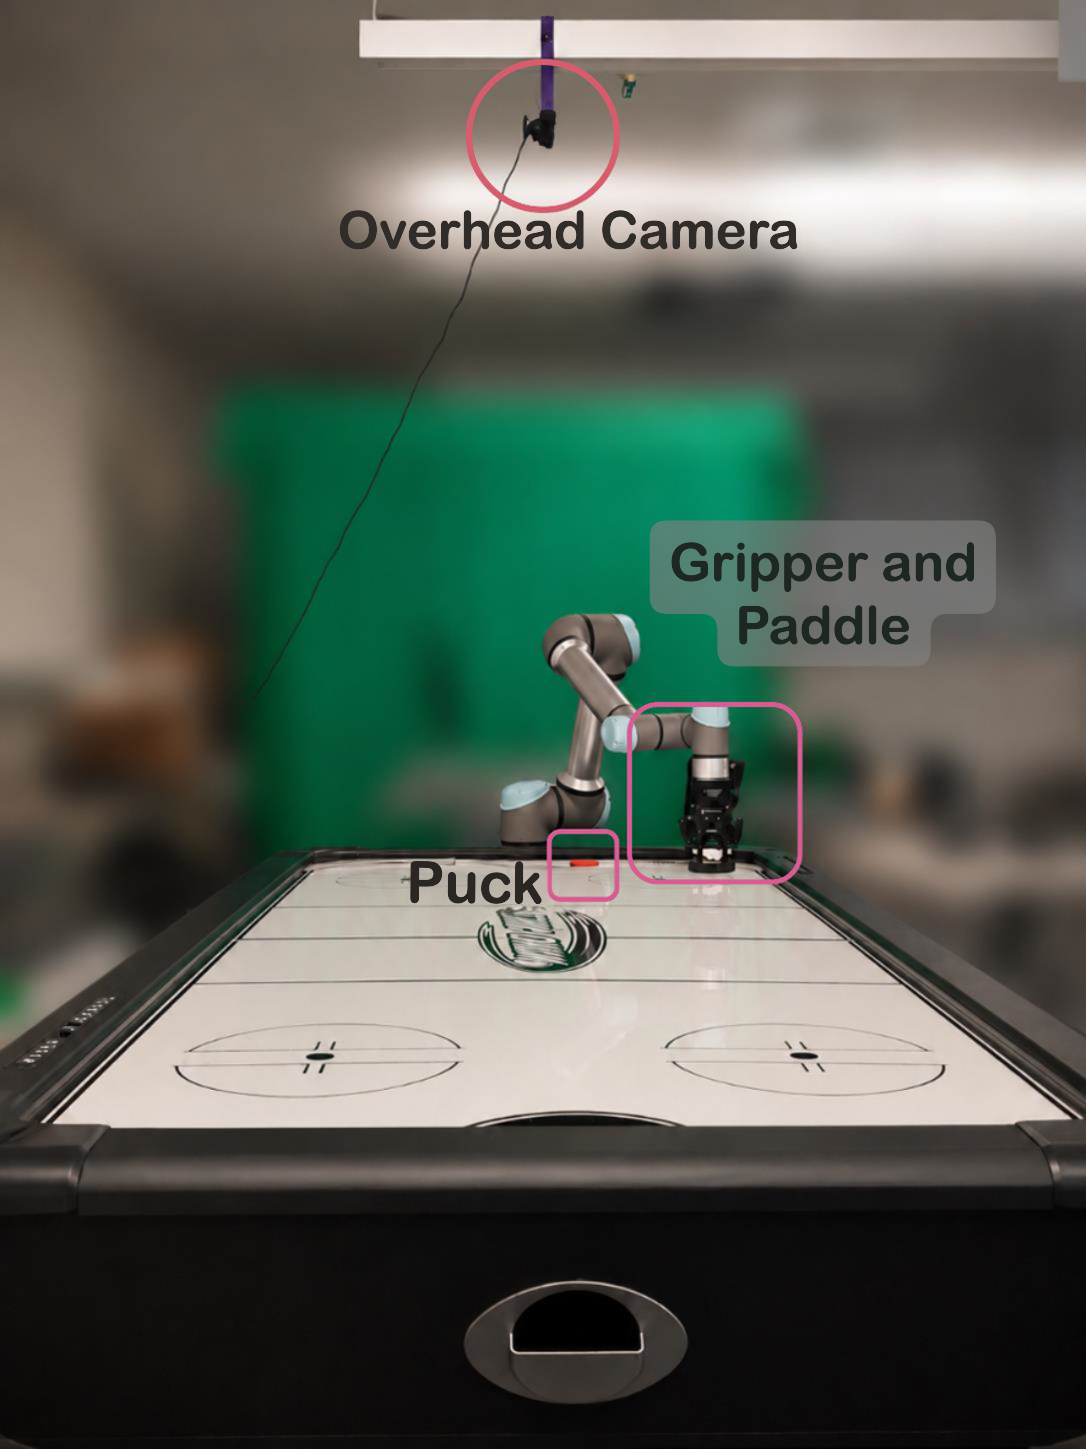
\includegraphics[width=0.38\textwidth]{figure/air_hockey_setup.png}
%     \caption{
%     Real-world robotic air hockey testbed.
%     }
%     \label{fig:real_world_air_hockey_setup}
%     \vspace{-1em}
% \end{wrapfigure}

Trajectories are as follows: after the puck successfully crosses the midline of the table, the learned policy begins until the puck falls to a position lower (closer to the base) than the robot. This pattern is akin to juggling, except that the task requires putting the radius of the puck inside the radius of the goal position (success), before the puck falls past the paddle (failure). Evaluation utilizes a fixed set of 20 goals in a $4\times5$ pattern, with 5 goals per row and 4 rows getting progressively lower. Additional details, including the dimensions of the table, paddle, puck, etc., can be found in \citet{chuck2024robot}.

To transfer trained policies from the simulator to the real robot, we first identified system parameters for the paddle using a small number (2 min) of human-generated paddle data. Puck parameters are then estimated based on human juggling data and the physics of the puck, as this was superior to black box optimization for estimating these parameters. Consequently, a meaningful sim-to-real gap exists in the puck movement between the real and simulated environments. To train policies robust to this gap, we leverage domain randomization in the style of \citet{tobin2017domain,peng2018sim,kumar2021rma}. For system parameters, we randomize the paddle density (which affects collisions), puck damping, and gravity as follows: 
\begin{center}
\small
\begin{tabular}{lccc}
\hline
\textbf{Parameter} & \textbf{Range} & \textbf{SysID} & \textbf{Variation} \\
\hline
Paddle density & $[2250.0,\ 3750.0]$ & $3000$ & $\pm 25\%$ \\
Puck damping & $[0.1335,\ 0.2225]$ & $0.178$ & $\pm 25\%$ \\
Gravity & $[-0.826,\ -0.496]$ & $-0.661$ & $\pm 25\%$ \\
\hline
\end{tabular}
\end{center}

We also perform substantial random resets for the puck reset, resetting the puck at positions across the top and middle with randomly selected velocities, as well as random positions near the paddle, to simulate the variance and challenging positions from where a trajectory might start. The puck is also spawned in random positions across its workspace. Random Noise and occlusions (missing values) are added to the observation of the puck position to force the policy to be robust to perceptual noise, as well as adding perceptual delay, where the puck position is lagged when given to the agent. Finally, 4-step smoothing is applied to the real robot, and the movement of the paddle in simulation is tuned with a PID controller to match this kind of smooth motion. 

\begin{figure}[t]
    \centering
    \begin{subfigure}[t]{0.42\textwidth}
        \centering
        \includegraphics[width=\linewidth]{figure/real_folder/trajectory_plot/crtr_trajectory_plot_goal_selector.png}
        \caption{Trajectory-space visualization.}
        \label{fig:crtr-trajectory}
    \end{subfigure}
    \hfill
    \begin{subfigure}[t]{0.42\textwidth}
        \centering
        \includegraphics[width=\linewidth]{figure/real_folder/long_exposure/crtr_goal_selector.png}
        \caption{Long-exposure real-world rollout.}
        \label{fig:crtr-long-exposure}
    \end{subfigure}
    \caption{CRTR evaluation rollouts across 20/20 achieved goals.}
    \label{fig:crtr-paired}
\end{figure}


% -----------------------------
% IWR Render
% -----------------------------
\begin{figure}[t]
    \centering
    \begin{subfigure}[t]{0.42\textwidth}
        \centering
        \includegraphics[width=\linewidth]{figure/real_folder/trajectory_plot/iwr_render_trajectory_plot_goal_selector.png}
        \caption{Trajectory-space visualization.}
        \label{fig:iwr-render-trajectory}
    \end{subfigure}
    \hfill
    \begin{subfigure}[t]{0.42\textwidth}
        \centering
        \includegraphics[width=\linewidth]{figure/real_folder/long_exposure/iwr_render_goal_selector.png}
        \caption{Long-exposure real-world rollout.}
        \label{fig:iwr-render-long-exposure}
    \end{subfigure}
    \caption{IWR evaluation rollouts across 20/20 achieved goals.}
    \label{fig:iwr-render-paired}
\end{figure}


% -----------------------------
% PPO
% -----------------------------
\begin{figure}[t]
    \centering
    \begin{subfigure}[t]{0.42\textwidth}
        \centering
        \includegraphics[width=\linewidth]{figure/real_folder/trajectory_plot/ppo_trajectory_plot_goal_selector.png}
        \caption{Trajectory-space visualization.}
        \label{fig:ppo-trajectory}
    \end{subfigure}
    \hfill
    \begin{subfigure}[t]{0.42\textwidth}
        \centering
        \includegraphics[width=\linewidth]{figure/real_folder/long_exposure/ppo_goal_selector.png}
        \caption{Long-exposure real-world rollout.}
        \label{fig:ppo-long-exposure}
    \end{subfigure}
    \caption{PPO evaluation rollouts across 20/20 achieved goals.}
    \label{fig:ppo-paired}
\end{figure}


% -----------------------------
% SAC-GCRL
% -----------------------------
\begin{figure}[t]
    \centering
    \begin{subfigure}[t]{0.42\textwidth}
        \centering
        \includegraphics[width=\linewidth]{figure/real_folder/trajectory_plot/sac_gcrl_trajectory_plot_goal_selector.png}
        \caption{Trajectory-space visualization.}
        \label{fig:sac-gcrl-trajectory}
    \end{subfigure}
    \hfill
    \begin{subfigure}[t]{0.42\textwidth}
        \centering
        \includegraphics[width=\linewidth]{figure/real_folder/long_exposure/sac_gcrl_goal_selector.png}
        \caption{Long-exposure real-world rollout.}
        \label{fig:sac-gcrl-long-exposure}
    \end{subfigure}
    \caption{SAC-GCRL evaluation rollouts across 20/20 achieved goals.}
    \label{fig:sac-gcrl-paired}
\end{figure}


% -----------------------------
% SAC-HER
% -----------------------------
\begin{figure}[t]
    \centering
    \begin{subfigure}[t]{0.42\textwidth}
        \centering
        \includegraphics[width=\linewidth]{figure/real_folder/trajectory_plot/sac_her_trajectory_plot_goal_selector.png}
        \caption{Trajectory-space visualization.}
        \label{fig:sac-her-trajectory}
    \end{subfigure}
    \hfill
    \begin{subfigure}[t]{0.42\textwidth}
        \centering
        \includegraphics[width=\linewidth]{figure/real_folder/long_exposure/sac_her_goal_selector.png}
        \caption{Long-exposure real-world rollout.}
        \label{fig:sac-her-long-exposure}
    \end{subfigure}
    \caption{SAC-HER evaluation rollouts across 20/20 achieved goals.}
    \label{fig:sac-her-paired}
\end{figure}


% -----------------------------
% SAC-Hint
% -----------------------------
\begin{figure}[t]
    \centering
    \begin{subfigure}[t]{0.42\textwidth}
        \centering
        \includegraphics[width=\linewidth]{figure/real_folder/trajectory_plot/sac_hint_trajectory_plot_goal_selector.png}
        \caption{Trajectory-space visualization.}
        \label{fig:sac-hint-trajectory}
    \end{subfigure}
    \hfill
    \begin{subfigure}[t]{0.42\textwidth}
        \centering
        \includegraphics[width=\linewidth]{figure/real_folder/long_exposure/sac_hint_goal_selector.png}
        \caption{Long-exposure real-world rollout.}
        \label{fig:sac-hint-long-exposure}
    \end{subfigure}
    \caption{SAC-Hint evaluation rollouts across 20/20 achieved goals.}
    \label{fig:sac-hint-paired}
\end{figure}


% -----------------------------
% SGCRL Render
% -----------------------------
\begin{figure}[t]
    \centering
    \begin{subfigure}[t]{0.42\textwidth}
        \centering
        \includegraphics[width=\linewidth]{figure/real_folder/trajectory_plot/sgcrl_render_trajectory_plot_goal_selector.png}
        \caption{Trajectory-space visualization.}
        \label{fig:sgcrl-render-trajectory}
    \end{subfigure}
    \hfill
    \begin{subfigure}[t]{0.42\textwidth}
        \centering
        \includegraphics[width=\linewidth]{figure/real_folder/long_exposure/sgcrl_render_goal_selector.png}
        \caption{Long-exposure real-world rollout.}
        \label{fig:sgcrl-render-long-exposure}
    \end{subfigure}
    \caption{SGCRL evaluation rollouts across 20/20 achieved goals.}
    \label{fig:sgcrl-render-paired}
\end{figure}